\documentclass[10pt,a4paper]{article}
\usepackage[utf8]{inputenc}
\usepackage{amsmath}
\usepackage{amsfonts}
\usepackage{amssymb}
\usepackage{hyperref}

\usepackage{graphicx}
\graphicspath{ {./images/} }

\hypersetup{
    colorlinks=true,
    linkcolor=blue,
    filecolor=magenta,      
    urlcolor=cyan,
    pdftitle={Overleaf Example},
    pdfpagemode=FullScreen,
    }

\title{Chapter 2 - Multi-armed Bandits Answers}
\author{Stéphane Liem NGUYEN}
\begin{document}
\maketitle

Exercises with (\textbf{\textit{corrected}}) were corrected based on the \href{http://incompleteideas.net/book/errata.html}{Errata}.

These are my own answers and mistakes or errors are possible.

\paragraph{\textit{Exercise 2.1} (p. 28)} In $\epsilon$-greedy action selection, for the case of two actions and $\epsilon = 0.5$, what is
the probability that the greedy action is selected?

\bigskip
Recall that at each time step, $\epsilon$-greedy action selection methods select with probability $\epsilon$ a random action uniformly out of $k$ actions (if there's $k$ actions) and with probability $1-\epsilon$ one of the greedy actions with ties broken arbitrarily (for instance randomly).

From the recall, we can say that the probability of the greedy action to be selected   is $1-\epsilon = 0.5$.

\paragraph{\textit{Exercise 2.2: Bandit example} (p. 30)} Consider a $k$-armed bandit problem with $k = 4$ actions,
denoted $1$, $2$, $3$, and $4$. Consider applying to this problem a bandit algorithm using
$\epsilon$-greedy action selection, sample-average action-value estimates, and initial estimates
of $Q_1(a) = 0$, for all a. Suppose the initial sequence of actions and rewards is $A_1 = 1,
R_1 = -1, A_2 = 2, R_2 = 1, A_3 = 2, R_3 = -2, A_4 = 2, R_4 = 2, A_5 = 3, R_5 = 0$. On some of these time steps the $\epsilon$ case may have occurred, causing an action to be selected at
random. On which time steps did this definitely occur? On which time steps could this
possibly have occurred?

\bigskip
We already recalled what were the $\epsilon$-greedy action selection methods. We can recall quickly that sample-average action-value estimates compute estimates $Q_n(a)$ based on an empirical mean of the rewards received when the action $a$ is taken. The empirical means can be computed incrementally as explained in the book.

To know in what time step did the $\epsilon$ case definitely occur, we use the information that the decision-maker only picks a non-greedy action (not actions with highest current estimates) when exploring.

For this reason, we also compute estimates after each action-selection:
\begin{enumerate}
\item Take action $1$, receive reward $-1$ and update estimates with $Q_2(1)=-1$ and keep $Q_1(a)=0,\, \forall a \neq 1$. For the next action selection, the action $1$ cannot be selected from greedy selection because its estimate is lower than the rest. The action $1$ can only be picked from exploration for the next action selection.

\item Take action $2$, receive reward $1$ and update estimates with $Q_2(2)=1$ and keep $Q_2(1)=-1,\, Q_1(a)=0,\, \forall a \notin \{1, 2\}$. For the next time step, if we pick another action than $2$ then it would be due to exploration.

\item Take action $2$, receive reward $-2$ and update estimates with $Q_3(2)=\frac{1 + (-2)}{2} = -0.5$ and keep $Q_2(1)=-1,\, Q_1(a)=0,\, \forall a \notin \{1, 2\}$. For the next action selection, the action $2$ can only be picked from exploration because its estimate is lower than the estimates of actions $3$ and $4$.

\item Take action $2$, receive reward $2$ and update estimates with $Q_4(2)=\frac{1 + (-2) + 2}{3} = \frac{1}{3}$ and keep $Q_2(1)=-1,\, Q_1(a)=0,\, \forall a \notin \{1, 2\}$. For the next time step, if we pick another action than $2$ then it would be due to exploration. 

\item Take action $3$, receive reward $0$ and update estimates with $Q_2(3)=0$ and keep $Q_4(2) = \frac{1}{3},\, Q_2(1)=-1,\, Q_1(4)=0$.

\end{enumerate}

The $\epsilon$ case could have occurred at all time steps but it definitely occurred  for time step $4$ and time step $5$.

\paragraph{\textit{Exercise 2.3} (p. 30)} In the comparison shown in Figure $2.2$, which method will perform best in
the long run in terms of cumulative reward and probability of selecting the best action?
How much better will it be? Express your answer quantitatively.

\bigskip
Action-value method with $\epsilon=0.01$ will perform best in the long run in terms of cumulative reward and probability of selecting the best action.

The probability of selecting the best action $a_*$ for $\epsilon$-greedy methods with $\epsilon > 0$ (with sample-averages and on stationary problems) can be written as the probability of taking an optimal action when exploring ($\epsilon$ case, action selected at random) plus the probability of taking a greedy action (we can add them because in one single action selection, we cannot behave greedily at the same time as non-greedily. Moreover the second part with greedy action assumes that the estimates of the optimal actions converge to the action values).

\begin{equation}
\lim_{t\to\infty}\mathbb{P}[A_t = a_*] = \epsilon\cdot\frac{1}{k}+ 1 - \epsilon
\end{equation}

This formula does not work for $\epsilon = 0$ (greedy) because if $\epsilon=0$, some actions can be selected a finite number of times asymptotically. As consequence, some estimates might not converge to the true action values.

For $10$-armed testbed, $k=10$ and by applying the formula with $\epsilon=0.1$ we get $0.01 + 1 - 0.1 = 0.91$. If we apply the formula with $\epsilon=0.01$ then we get $0.001 + 1 - 0.01 = 0.991$.

\clearpage
\paragraph{\textit{Exercise 2.4} (p. 33)} If the step-size parameters, $\alpha_n$, are not constant, then the estimate $Q_n$ is
a weighted average of previously received rewards with a weighting different from that
given by ($2.6$). What is the weighting on each prior reward for the general case, analogous
to ($2.6$), in terms of the sequence of step-size parameters?

\bigskip
Recall that in this section, the book focused on estimating/tracking incrementally the value of a single action for nonstationary problem and this was done by using a constant-step-size parameter in the incremental update rule that we rewrite below
\begin{equation}
Q_{n+1} \doteq Q_n + \alpha_n [R_n - Q_n]
\end{equation}
where $R_n$ is the reward received after the $n$-th selection of the action and $\alpha_n=\frac{1}{n}$ for the incremental implementation of sample-averages (empirical mean) or $\alpha_n=\alpha \in (0, 1]$ for the exponential recency-weighted average.

Equation $(2.6)$ showed that if we update estimates using exponential recency-weighted average then $Q_{n+1}$ was a weighted average of past rewards and the initial estimate $Q_1$.

We can try to do the same but for the general case where $\alpha_n$ is not necessarily $\frac{1}{n}$ or a constant $\alpha \in (0,1]$.
\begin{equation}
\begin{split}
Q_{n+1} &= Q_n + \alpha_n [R_n - Q_n] = \alpha_n R_n + (1-\alpha_n) Q_n\\
&= \alpha_n R_n + (1-\alpha_n) [\alpha_{n-1} R_{n-1} + (1-\alpha_{n-1})Q_{n-1}]\\
&= \alpha_n R_n + (1-\alpha_n) \alpha_{n-1} R_{n-1} + (1-\alpha_n)\cdot (1-\alpha_{n-1})Q_{n-1}\\
&= Q_1 \prod_{k=1}^n (1-\alpha_k) + \sum_{i=1}^n \alpha_i R_i \prod_{j=i+1}^n (1-\alpha_j)
\end{split}
\end{equation}

Each reward $R_i$ is weighted by $\alpha_i \prod_{j=i+1}^n (1-\alpha_j)$.

\bigskip
We can verify by recurrence that it's a weighted sum, i.e $\prod_{k=1}^n (1-\alpha_k) + \sum_{i=1}^n \alpha_i \prod_{j=i+1}^n (1-\alpha_j) = 1$. For $n=1$ we have
\begin{equation}
1-\alpha_1 + \alpha_1 = 1
\end{equation}
Suppose the formula is true for $n$, let's prove that it holds for $n+1$. Let $H_n = \prod_{k=1}^n (1-\alpha_k) + \sum_{i=1}^n \alpha_i \prod_{j=i+1}^n (1-\alpha_j) = 1$

\begin{equation}
\prod_{k=1}^{n+1} (1-\alpha_k) + \sum_{i=1}^{n+1} \alpha_i \prod_{j=i+1}^{n+1} (1-\alpha_j) = H_n \cdot (1-\alpha_{n+1}) + \alpha_{n+1} = 1
\end{equation}

From the general formula, we can obtain equation $(2.6)$ of the book for exponential recency-weighted average as well as the sample-average methods where $R_i$'s are weighted by $\frac{1}{i} \cdot \prod_{j=i+1}^n \left(1-\frac{1}{j}\right) = \frac{1}{i} \cdot \frac{n-1}{n} \cdot \frac{n-2}{n-1} \cdot \hdots \cdot \frac{i}{i+1} = \frac{1}{n}$

\clearpage
\paragraph{\textit{Exercise 2.5 (programming)} (p. 33)} Design and conduct an experiment to demonstrate the
difficulties that sample-average methods have for nonstationary problems. Use a modified version of the $10$-armed testbed in which all the $q_*(a)$ start out equal and then take independent random walks (say by adding a normally distributed increment with mean $0$ and standard deviation $0.01$ to all the $q_*(a)$ on each step). Prepare plots like Figure $2.2$
for an action-value method using sample averages, incrementally computed, and another action-value method using a constant step-size parameter, $\alpha = 0.1$. Use $\epsilon = 0.1$ and
longer runs, say of 10,000 steps.

\bigskip
\begin{figure}[h]
\centering
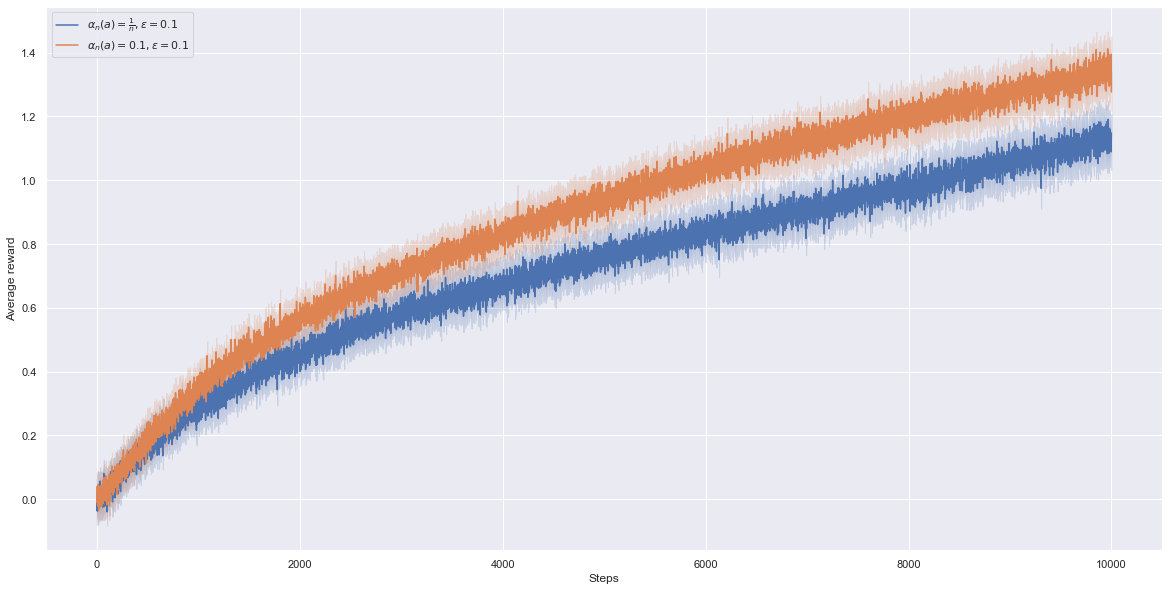
\includegraphics[width=\textwidth]{./non-stationary-testbed/images/avg_reward.png}
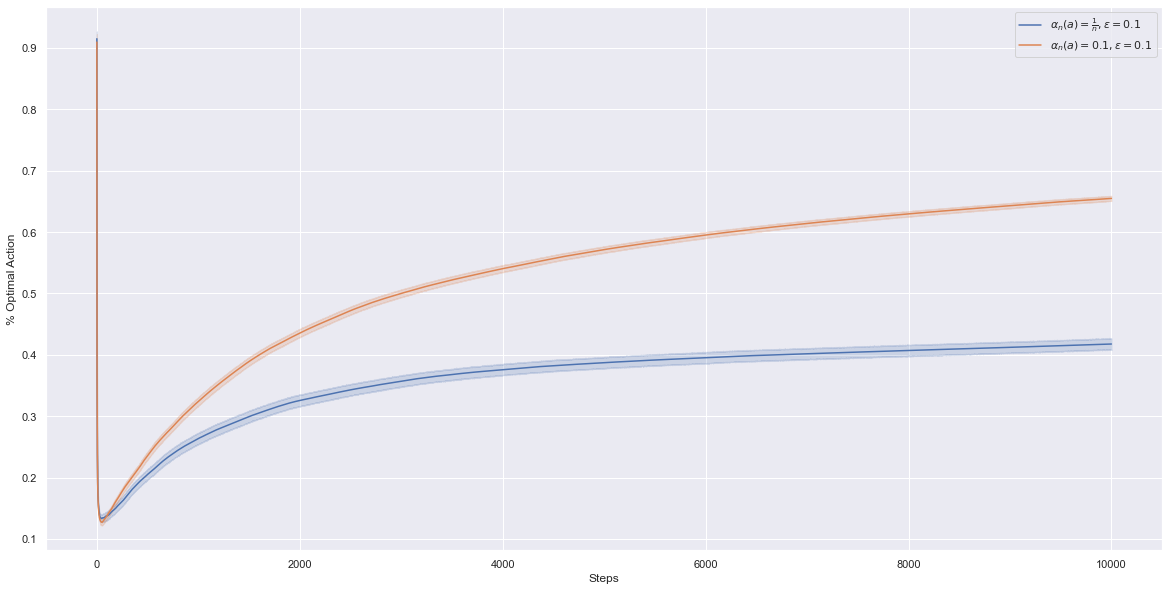
\includegraphics[width=\textwidth]{./non-stationary-testbed/images/percent_optimal_action.png}
\caption{Average performance of $\epsilon$-greedy action-value methods with different action-value estimates on a modified version of the 10-armed testbed with nonstationary reward distributions.
These data are averages over $2000$ runs with different nonstationary bandit problems and with longer runs of $10000$ steps. All methods used $\epsilon=0.1$ and we compared the sample-average methods with the exponential recency-weighted average method for estimating values.}
\end{figure}
We can observe that the sample-average methods struggle to track the optimal action that can change over time compared to exponential recency-weighted average that gives more weight to recent rewards than old rewards. The code for the exercise can be found \href{https://github.com/Zenchiyu/learning-rl/tree/develop/Intro_RL_Sutton_book/Chap2-Multi-Armed-Bandits/non-stationary-testbed#non-stationary-testbed}{here}.

\paragraph{\textit{Exercise 2.6: Mysterious Spikes} (p. 35)} The results shown in Figure $2.3$ should be quite reliable because they are averages over $2000$ individual, randomly chosen $10$-armed bandit tasks.
Why, then, are there oscillations and spikes in the early part of the curve for the optimistic method? In other words, what might make this method perform particularly better or worse, on average, on particular early steps?

\bigskip
In the book, optimistic initial action-value estimates method was applied on stationary problems (reward distributions do not change over time) and we track action-values by exponential recency-weighted average (constant step-size parameter) to use the bias caused by initial estimates (if we used sample-averages, the bias disappears once all actions are selected at least once).

For the first $k$ action-selections, the method (with greedy selections) explored most of the time all the existing actions because the initial estimates are optimistic compared to the reward distributions with means given by a standard normal distribution (rewards received are most of the time lower than $5$). Consequently, the percentage of action selections out of $2000$ runs that are optimal are initially around $10$ percent ($1/k=0.1$ for $k=10$).

After the $k$ first action-selections, all action selections are based on estimates computed from a weighted sum of past rewards and initial estimates of $5$ where the bias decreases over time as well as the exploration.

The mysterious spikes come from the frequent selection of the optimal action just after the first $k$ action selections. This might be due the first reward of the optimal action (obtained most of the time from the $k$ first action selections) that can be in average higher sometimes than the rest and this implies a higher $Q_2(a)$ for the optimal action. After the selection of the optimal action, the impact of the initial estimate and the estimates of the action value for the action are both reduced. This gives more chance for the other non optimal actions to be selected.


\paragraph{\textit{Exercise 2.7: Unbiased Constant-Step-Size Trick} (\textit{corrected}) (p. 35)} In most of this chapter we have used
sample averages to estimate action values because sample averages do not produce the
initial bias that constant step sizes do (see the analysis leading to ($2.6$)). However, sample averages are not a completely satisfactory solution because they may perform poorly on nonstationary problems. Is it possible to avoid the bias of constant step sizes while retaining their advantages on nonstationary problems? One way is to use a step size of
\begin{equation}
\beta_n \doteq \alpha/\bar{o}_n
\end{equation}

to process the $n$th reward for a particular action, where $\alpha > 0$ is a conventional constant step size, and $\bar{o}_n$ is a trace of one that starts at $0$:
\begin{equation}
\bar{o}_n \doteq \bar{o}_{n-1} + \alpha \cdot (1 - \bar{o}_{n-1}),\quad \textrm{for } n > 0,\quad \textrm{with } \bar{o}_0 \doteq 0
\end{equation}

Carry out an analysis like that in ($2.6$) to show that $Q_n$ is an exponential recency-weighted average \textit{without initial bias}.

\bigskip
With the unbiased constant-step-size trick, the step size parameter $\beta_n$ starts at $1$ and decreases until it reaches the constant step size $\alpha \in (0, 1]$. Because it starts at $1$, the initial bias disappears once all actions are selected at least once. Moreover, because the step size parameter doesn't decrease below $\alpha$, we obtain some advantages of exponential recency-weighted average for tracking nonstationary problems.

We start to plugging the new step size into the incremental update rule and then carry out an analysis like ($2.6$) of the book.
\begin{equation}\label{ex_2_7_incr_update_rule}
\begin{split}
Q_{n+1} &\doteq Q_n + \beta_n [R_n - Q_n],\quad \beta_n \doteq \alpha/\bar{o}_n\\
&=Q_1 \prod_{k=1}^n (1-\beta_k) + \sum_{i=1}^n \beta_i R_i \prod_{j=i+1}^n (1-\beta_j)\\
&=Q_1 \cdot (1 - \beta_1) \prod_{k=2}^n (1-\beta_k) + \sum_{i=1}^n \beta_i R_i \prod_{j=i+1}^n (1-\beta_j)\\
&= \sum_{i=1}^n \beta_i R_i \prod_{j=i+1}^n (1-\beta_j) = \sum_{i=1}^n \frac{\alpha}{\bar{o}_i} R_i \prod_{j=i+1}^n (1-\frac{\alpha}{\bar{o}_j})
\end{split}
\end{equation}
by using $\beta_1 = \alpha/\alpha = 1$ because $\bar{o}_1 = \alpha$. Each reward $R_i$ is weighted by $\frac{\alpha}{\bar{o}_i} \prod_{j=i+1}^n (1-\frac{\alpha}{\bar{o}_j})$.

If we try to apply the same procedure (or substitute in ($2.6$) of the book) but on the trace of one we get
\begin{equation}
\begin{split}
\bar{o}_n = \sum_{k=0}^{n-1} (1-\alpha)^k \alpha,\quad \textrm{for } n > 0,\quad \textrm{with } \bar{o}_0 \doteq 0
\end{split}
\end{equation}
and this converges to $1$ (geometric series). So as $n \to \infty$, the weights on each reward are like exponential recency-weighted average.

%Substituting that back into our equation \ref{ex_2_7_incr_update_rule} gives
%\begin{equation}
%Q_{n + 1} = \sum_{i=1}^n \frac{\alpha}{\bar{o}_i} R_i \prod_{j=i+1}^n (1-\frac{\alpha}{\bar{o}_j})
%\end{equation}


\paragraph{\textit{Exercise 2.8: UCB Spikes} (p. 36)} In Figure $2.4$ the UCB algorithm shows a distinct spike
in performance on the $11$th step. Why is this? Note that for your answer to be fully satisfactory it must explain both why the reward increases on the $11$th step and why it decreases on the subsequent steps. Hint: If $c = 1$, then the spike is less prominent.

\paragraph{\textit{Exercise 2.9} (p. 37)} Show that in the case of two actions, the soft-max distribution is the same
as that given by the logistic, or sigmoid function often used in statistics and artificial
neural networks.

\bigskip
We can first recall the formula for the soft-max distribution based on action preferences
\begin{equation}
\mathbb{P}[A_t = a] \doteq \frac{e^{H_t(a)}}{\sum_{b=1}^k H_t(b)} \doteq \pi_t(a)
\end{equation}
where $H_t(a)$ is the numerical \textit{preference} of action $a$.

And for two actions $1$ and $2$, we have
\begin{equation}
\mathbb{P}[A_t = 1] = \frac{e^{H_t(1)}}{ e^{H_t(1)} + e^{H_t(2)}} = \frac{1}{1 +  e^{H_t(2) -  H_t(1)}} = \frac{1}{1 +  e^{-x}}
\end{equation}
with $x = H_t(1)- H_t(2)$

\paragraph{\textit{Exercise 2.10} (p. 41)} Suppose you face a $2$-armed bandit task whose true action values change randomly from time step to time step. Specifically, suppose that, for any time step, the true values of actions $1$ and $2$ are respectively $10$ and $20$ with probability $0.5$ (case
A), and $90$ and $80$ with probability $0.5$ (case B). If you are not able to tell which case you face at any step, what is the best expected reward you can achieve and how should you behave to achieve it?

Now suppose that on each step you are told whether you are facing case A or case B (although you still don't know the true action values). This is an associative search task. What is the best expected reward you can achieve in this task, and how should you behave to achieve it?

\bigskip
If we're not able to tell which case we face at any step, then the problem can be converted into a single stationary $2$-armed bandit task where the true values of the actions would be $(10 + 90)/2 = 50$ for action $1$ and $(20 + 80)/2 = 50$ for action $2$. The best expected reward we can achieve would be $50$. We can behave either randomly by selecting actions uniformly or always pick the first action or always pick the second action.

If we know what case we face at each step, the best expected reward we can achieve would be $(20 + 90)/2=55$ by taking action $2$ when we face case A and by taking action $1$ when we face case B.


\paragraph{\textit{Exercise 2.11 (programming)} (p. 44)} Make a figure analogous to Figure $2.6$ (parameter study) for the nonstationary case outlined in \textbf{\textit{Exercise 2.5}}. Include the constant-step-size $\epsilon$-greedy algorithm with
$\alpha=0.1$. Use runs of 200,000 steps and, as a performance measure for each algorithm and parameter setting, use the average reward over the last 100,000 steps.
\end{document}